\section{Model Room Illuminance Calculation}
The algorithm was tested on model room of dimension $\left(10 \times 5 \times 4\right)$~m. Any barriers or equipment were not considered. Pure diffuse reflections were considered with facets reflectance:
\begin{itemize}
	\item $\rho = 0.2$ for floor,
	\item $\rho = 0.5$ for walls,
	\item $\rho = 0.7$ for ceiling.
\end{itemize}
Each facet has the same dimension $\left(0.25 \times 0.25\right)$~m. $4$~reflections were evaluated for each solution. High count of reflection slows down the algorithm. It was found out that there was increase less than $10$~\% in resulting illuminance after the 4\textsuperscript{th} reflection. This fact was tested in simulation after only one lamp was presented in the middle of the rooms ceiling. The result is graphically shown in Figure~\ref{fig:reflDif}.

\begin{figure}[htb]
  \centering
  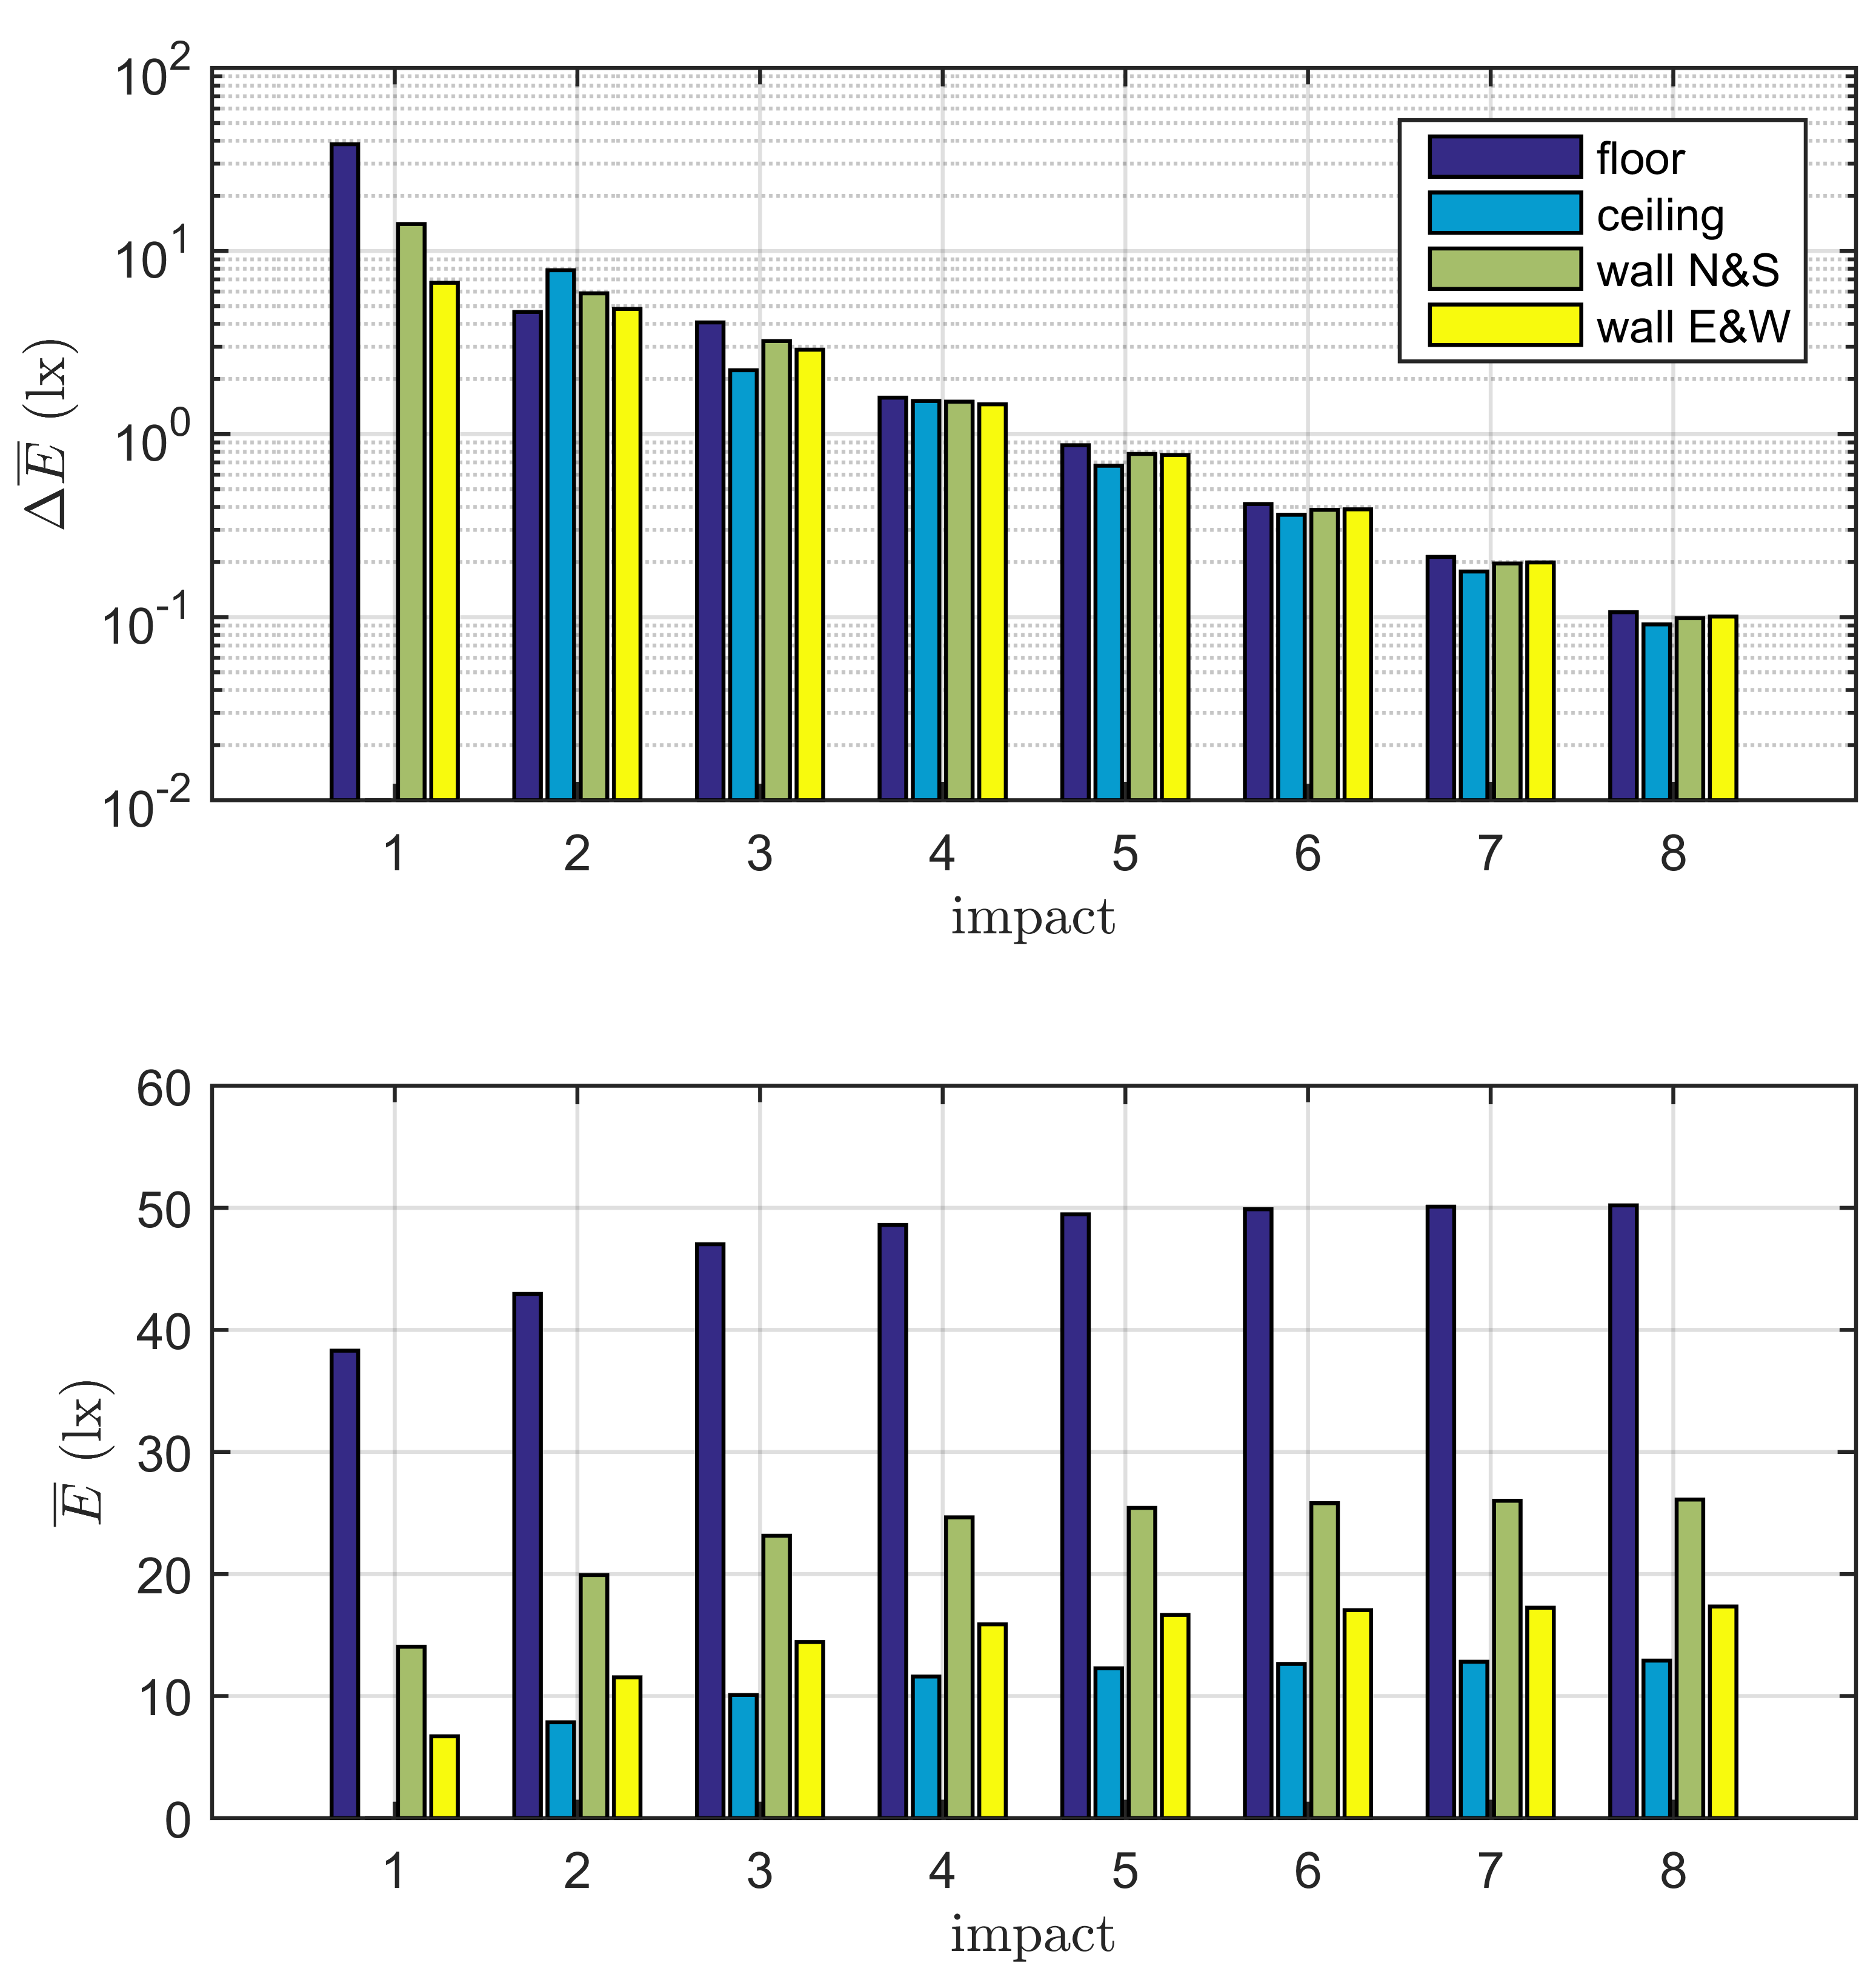
\includegraphics[width=\columnwidth]{reflDif}
  \caption{Increase of the wall average illuminance for one lamp in the room ceiling center according to the count of reflections.}
  \label{fig:reflDif}
\end{figure}

The grid of control points was placed on reference plane with distances 25~cm.